\documentclass{article}

% NeurIPS 2025 — default (anonymized review) mode.
% Switch to \usepackage[preprint]{neurips_2025} to deanonymize.
\usepackage{neurips_2025}

\usepackage[utf8]{inputenc}
\usepackage[T1]{fontenc}
\usepackage{amsmath,amssymb}
\usepackage{graphicx}
\usepackage{booktabs}
\usepackage{subcaption}
\usepackage{xcolor}
\usepackage{url}
\usepackage{microtype}
\usepackage{tikz}
\usetikzlibrary{arrows.meta,positioning,shapes.geometric}

\graphicspath{{figures/out/}}

\newcommand{\pres}[2]{\langle #1 \mid #2 \rangle}
\newcommand{\AK}{\mathrm{AK}}
\newcommand{\MS}{\mathrm{MS}}
\newcommand{\Ffloor}{F}

\title{The Hump, Not the Cap: A Negative-Result Audit and a Structural
  Floor for the Stable Andrews--Curtis Conjecture on $\AK(3)$}

% Review mode: the style prints "Anonymous Author(s)".
\author{%
  Anonymous Author(s)\\
  Affiliation\\
  \texttt{email}\\
}

\begin{document}

\maketitle

\begin{abstract}
\input{sections/00_abstract}
\end{abstract}

\section{Introduction}\label{sec:intro}

The Andrews--Curtis (AC) conjecture \cite{andrews1965ac} states that every \emph{balanced}
presentation of the trivial group --- a presentation $\langle x_1,\dots,x_n \mid
r_1,\dots,r_n\rangle$ with as many relators as generators that presents the one-element
group --- can be transformed into the trivial presentation $\langle x_1,\dots,x_n \mid
x_1,\dots,x_n\rangle$ by a finite sequence of elementary moves. Sixty years after it was
posed, it remains open, and its difficulty is not merely combinatorial folklore: a
balanced presentation that resisted trivialization would refute the conjecture, and the
same balanced presentations sit at the heart of low-dimensional topology, where they
encode handle decompositions of contractible $4$-manifolds. Potential AC counterexamples
arise directly from Akbulut--Kirby's smooth $4$-dimensional constructions
\cite{akbulut1985ac} and from candidate counterexamples to the Property $2R$ and
slice--ribbon conjectures \cite{gompf2010fibered}, and the conjecture is explicitly
entangled with the smooth $4$-dimensional Poincar\'e problem \cite{freedman2010poincare}.
Among all candidates, the Akbulut--Kirby presentation $\mathrm{AK}(3) = \langle x,y \mid
x^{3}=y^{4},\ xyx=yxy\rangle$ is the shortest and most-studied potential counterexample,
standing since 1985.

The \emph{stable} (or \emph{weak}) AC conjecture relaxes the problem by allowing two
further moves, stabilization by a trivial generator--relator pair (AC4) and its inverse
(AC5); a presentation reducible to the trivial one under AC1--AC5 is \emph{stably
AC-trivial}. The stable status of $\mathrm{AK}(3)$ has recently oscillated. The first
version of a 2024 case study \cite{shehper2024hard} announced that $\mathrm{AK}(3)$ is
stably AC-trivial, removing it as a stable-AC counterexample; a subsequent revision
located a misprint in the Wirtinger construction of \cite{myasnikov2002ac} on which that
argument depended and rescinded the claim. A parallel automated-deduction paper
\cite{lisitsa2025ak3}, written between those two versions, builds its stable-triviality
conclusion on the same, now-rescinded premise and has not been revised. The plain reading
of the current literature is therefore blunt: the stable AC-triviality of $\mathrm{AK}(3)$
is open again.

Search-based and learning-based methods have crossed hard barriers in this domain before
--- genetic algorithms trivialized $\mathrm{AK}(2)$ \cite{miasnikov1999genetic}, and a
recent study of the AC difficulty landscape \cite{fagan2026twohump} pushed reinforcement
learning past presentations that classical search cannot reach. This invites a concrete
question about stabilization as an escape hatch: does adding a generator $z$ defined by a
relator $z^{-1}w(x,y)$ --- for a cleverly chosen word $w$ in the original generators --- open
shortcuts (informally, ``wormholes'') through the enlarged AC graph that ordinary
2-generator search cannot find? If some $w$ trivialized $\mathrm{AK}(3)$ where the dumb
choices $z=r_i$ do not, stabilization would be a genuine algorithmic lever rather than
bookkeeping.

This paper is a systematic audit of that hope, and it returns a rigorously verified
negative paired with a structural map (Figure~\ref{fig:overview}). We first re-verify,
seven independent ways, that the stable status of $\mathrm{AK}(3)$ is open while its
plain-AC equivalence to the length-25 presentation P25 survives. We then run three
stabilization strategies of increasing sophistication --- all of which fail within the
searched budgets --- and a control showing that the per-relator length cap is not what stops
them. Finally, we characterize \emph{where} stabilized greedy search stalls: a length-13
floor whose AC-class has exactly two canonical representatives, bridged by a certified
move sequence. Throughout, every positive claim is emitted as a machine-checkable
certificate.

\begin{figure}[t]
\centering
\resizebox{\textwidth}{!}{%
\begin{tikzpicture}[
  font=\small,
  box/.style={draw, rounded corners, align=center, inner sep=5pt, fill=gray!12},
  attack/.style={draw, rounded corners, align=center, text width=33mm,
                 minimum height=11mm, inner sep=4pt, fill=gray!3},
  arr/.style={-{Latex[length=2.2mm]}, thick, gray!55},
]
\node[box, text width=30mm] (m)
  {\textbf{MMS02 misprint}\\$\to$ v2 rescission\\[2pt]$\mathrm{AK}(3)$ stable\\status re-opened\\(7/7 checks)};

\node[attack, right=17mm of m, yshift=15mm] (a1) {naive $z{=}w$ over 640 MS};
\node[attack, below=5mm of a1] (a2) {97-word bank on $\mathrm{AK}(3)$};
\node[attack, below=5mm of a2] (a3) {five lanes incl.\ Lemma-11 plateau elim.:\\180{,}645 quotients};

\node[draw, dashed, rounded corners, fit=(a1)(a2)(a3), inner sep=6pt,
      label={[font=\footnotesize]above:three stabilization attacks}] (grp) {};

\node[align=center, font=\footnotesize\bfseries, right=11mm of a2] (zero)
  {0 solved\\(within budget)};

\node[box, text width=24mm, right=8mm of zero] (cap)
  {\textbf{cap control}\\$L\le48$:\\not binding};

\node[box, text width=33mm, right=8mm of cap, fill=gray!22] (floor)
  {\textbf{length-13 floor}\\two canonical reps\\$F$ (71\%) / $\mathrm{AK}(3)$ (29\%)\\certified 21-move bridge};

\draw[arr] (m) -- (grp);
\draw[arr] (a1.east) -- (zero.north west);
\draw[arr] (a2.east) -- (zero.west);
\draw[arr] (a3.east) -- (zero.south west);
\draw[arr] (zero) -- (cap);
\draw[arr] (cap) -- (floor);
\end{tikzpicture}%
}
\caption{End-to-end audit pipeline: a greedy substitution solver, a stabilization move
that defines a fresh generator $z$ by a chosen word $w(x,y)$, a $97$-word
literature-grounded bank, and five attack lanes (meet-in-the-middle, direct stable-move
search, trivial-$z$ control, plateau elimination, and a zero-shot RL beam probe), with
every reported solution emitted as a machine-checkable certificate replayed by two
independent verifiers.}
\label{fig:overview}
\end{figure}

\paragraph{Contributions.}
\begin{itemize}
  \item \textbf{Re-verification of a re-opened question.} We computationally confirm, via
    7 of 7 agreeing independent checks (Smith normal form, Todd--Coxeter coset enumeration,
    and $S_3$-homomorphism counting among them), that $\mathrm{AK}(3)$'s stable status is
    open, that the plain-AC link $\mathrm{AK}(3)\sim\mathrm{P}25$ survives (53-move replay,
    plus validation of an independent Prover9 derivation), and we surface two data defects
    in a published trivialization artifact.
  \item \textbf{Systematic stabilization negatives at stated budgets.} Across a naive
    $z=w$ construction over 640 Miller--Schupp presentations, a 97-word literature-grounded
    bank on $\mathrm{AK}(3)$, and a five-lane campaign that mines 180{,}645 distinct
    2-generator quotients, 0 of 16{,}870 solve attempts succeed within the searched
    budgets (up to $2\times10^{6}$ nodes per search, beam width $\le 2048$).
  \item \textbf{A cap-not-binding control.} We show the $L=24$ per-relator length cap is
    not the binding constraint in the tested range: relaxing to $L\le 48$ (and total
    length $\le 60$) does not convert a single failure into a success.
  \item \textbf{A two-representative structural floor.} The length-13 floor of
    $\mathrm{AK}(3)$'s AC-class has exactly two canonical (signed-relabel) representatives
    --- $F=\langle x,y \mid y^{-2}xyx^{-2},\ y^{-3}x^{-2}yx\rangle$, a $2$-generator
    presentation AC-equivalent to $\mathrm{AK}(3)$ (712/1006 $=71\%$ of floor states), and
    $\mathrm{AK}(3)$'s own reduced form (294/1006 $=29\%$) --- joined by a certified 21-move
    AC path.
  \item \textbf{A certificate framework and reusable archive.} We release the acx-cert-v1
    machine-checkable certificate format with two independently authored verifiers
    (20{,}947 checks, 0 failures) and the full candidate-quotient archive, so every claim
    above is independently re-runnable.
\end{itemize}

Code, data, and all certificates will be released on acceptance.

\input{sections/02_background}
\input{sections/03_methods}
\section{Experiments and Results}\label{sec:results}

Every search below shares the greedy substitution solver, the stabilization move, and the
certificate format described in the methods; we report negatives strictly within the
searched budgets and emit every positive as a machine-checkable certificate
(Appendix~\ref{app:certs}). We first re-verify the literature status of AK(3), then run
stabilization strategies of increasing sophistication --- all failing within the searched
budgets --- add a control that the length cap is not what stops them, and finally give a
structural map of where the search stalls. Two scales recur and must not be conflated: a
fully local reproduction (a $1{,}006$-candidate floor census, $1{,}937$ solve attempts) and
the consolidated campaign archive ($180{,}645$ harvested quotients, $16{,}870$ attempts,
$6{,}058$ distinct candidates); we keep them separate throughout.

\subsection{Re-verifying the literature status of AK(3)}

Table~\ref{tab:litchecks} collects seven independent computational checks of the misprint
story, all $7/7$ passing (Smith-normal-form abelianization, Todd--Coxeter/Felsch coset
enumeration, and $S_3$-homomorphism counting whose CSP hom-counter is validated $4/4$
against brute force on synthetic triple-relator systems). The \emph{corrected} Wirtinger
presentation $W$ is genuine: deleting any single relator --- all $14$ deletions --- leaves a
presentation of $\mathbb{Z}$. The misprinted $W'$ provably is not: one single-relator
deletion yields a $B_3$ fingerprint ($12$ homomorphisms to $S_3$, $6$ of them non-abelian),
while a different deletion is $\mathbb{Z}$-consistent --- two deletions presenting
\emph{non-isomorphic} groups, which no Wirtinger presentation of any diagram can do. AK(3)
itself presents the trivial group (coset enumeration, order $1$), and the Wirtinger-derived
$M3$ presentation reduces under Lemma 11 with $z:=y^{-1}x$ exactly to P25, pinning the
commutator convention (convention B) of MMS02~\cite{myasnikov2002ac}. The printed $53$-move
Appendix-F sequence~\cite{shehper2024hard} replays exactly from P25 to AK(3) ($53$ steps,
$54$ states), reaching a peak total relator length of $25$ en route --- above the
length-$13$ floor of \S4.8. An independently published
trivialization~\cite{lisitsa_zenodo, lisitsa2025ak3} ($159$ transitions) validates at
cyclic-word granularity once two data defects are handled (one corrupt transition, bridged
by composing adjacent moves; one mislabeled conjugation direction). The consequence is
unambiguous: the plain-AC bridge $\mathrm{AK}(3)\sim\mathrm{P}25$ is solid, while the
claimed stable-triviality of AK(3) has no surviving support (Appendix~\ref{app:misprint}).

\begin{table}[tbp]
\centering
\caption{Seven independent computational checks (rows 1--7) of the MMS02 misprint account,
all passing, plus two certificate/log re-verifications (rows 8--9): the corrected
Wirtinger presentation is genuine, the misprinted $W'$ is not, and the plain-AC bridge
$\mathrm{P}25\sim\mathrm{AK}(3)$ survives.}
\label{tab:litchecks}
\small
\setlength{\tabcolsep}{3pt}%
\begin{tabular}{lll}
\toprule
Check & Method & Result \\
\midrule
Self-test: hom-counter & CSP hom-counter vs. brute-force cross-check on 4 synthetic triple-relator systems (n$\le$4 generators) & PASS (4/4 match) \\
Check 1: corrected-W, all 14 deletions & SNF abelianization + Felsch coset enumeration on each single-relator deletion of corrected W & PASS (14/14 present Z) \\
Check 2: misprinted-W is broken & S3 hom-counting gate: misprinted W' deletions \{7,14\} disagree (B3 vs Z) while corrected-W deletions \{7,12,14\} all agree (Z) & PASS (gate satisfied) \\
Check 3: AK(3) is trivial & Felsch coset enumeration of the trivial subgroup (index = group order) & PASS (order 1) \\
Check 4: M3 (Wirtinger) = P25 & Reduced-word match of the Wirtinger-derived M3 transcription against P25 under commutator convention B & PASS (convention B matches) \\
Check 5: corrected-W, 3-gen reduction & SNF + S3 hom-count + coset collapse of corrected-W's (x,y,z) 3-generator reduction & PASS (presents Z) \\
Check 6: Remark 17 conjugation convention & Conjugation-convention match (g t $g^{-1}$) of r1/r2 against Remark 17 & PASS (r1, r2 both match) \\
Appendix-F 53-move replay [cert] & Replay of the printed AC' h-move sequence (Appendix F, arXiv:2408.15332v2), forward order/forward moves, from P25 & Lands exactly on AK(3) (53 steps, 54 states; cert appendixF\_P25\_to\_AK3.json) \\
Lisitsa S2 external replay [log] & Independent replay of Zenodo 14567743's 159-transition AC path P25$\to$AK(3) & PASS --- genuine bridge; 2 data defects found in the published artifact (line 91 corrupt relator, line 81 CONJ label swapped) \\
\bottomrule
\end{tabular}

\vspace{2pt}
{\footnotesize
Rows 1-7 are read verbatim from results/stable\_ac/ak3\_stable\_proof/literature\_checks.json (7 entries, all pass:true). Raw JSON key names differ in spelling/case from this table's human-readable labels; see the run report for the exact key list.\par
Rows 8-9 are additional re-verifications NOT drawn from literature\_checks.json: row 8 is sourced from the certificate results/stable\_ac/ak3\_stable\_proof/certs/appendixF\_P25\_to\_AK3.json (steps count read live from the cert); row 9 is sourced from the campaign log experiments/stable\_ac/ak3\_stable\_proof/RESULTS.md, section 'PL(partial) -- Lisitsa S2 independently validated'.\par
Key-name check: this table's originally-expected key spellings ['check3\_ak3\_trivial', 'check4\_M3\_lemma11\_P25', 'check5\_corrected\_family\_Z'] do not appear verbatim in literature\_checks.json; the actual keys (used above) are ['check3\_AK3\_trivial', 'check4\_M3\_to\_P25', 'check5\_correctedW\_3gen'].\par
}

\end{table}

\subsection{Naive $z=w$ stabilization does not extend the baseline}

Our reference point is the $640$ known-solvable MS(1190) presentations~\cite{miller1999ms}
($634$ solve under the per-relator cap $L=24$ at $10^6$ nodes; the remaining $6$ only under
the original sum cap). We stabilize each with a single defined generator $z=w$ and
re-solve, for $w\in\{r_1,r_2,x,y\}$, at $5\times10^5$ nodes (Figure~\ref{fig:arms},
Table~\ref{tab:arms}). Solved counts fall monotonically --- $619$ ($r_1$), $602$ ($r_2$),
$540$ ($x$), $523$ ($y$) --- with $21/38/100/117$ attempts budget-exhausted. Crucially, every
arm's solved set is a \emph{strict subset} of the baseline's: computed row-by-row,
$|\text{arm}\setminus\text{baseline}|=0$ for all four, the union across arms is $620$
(below the baseline $634$) and the intersection is $523$. Stabilization with a defined
generator thus reproduces, but never extends, the baseline within the searched budgets.
Median node counts stay small (baseline $11$; $r_1,r_2$ each $13$; $x,y$ each $10$), yet
the $x$ and $y$ arms' \emph{mean} nodes inflate to $14{,}681$ and $21{,}833$: defining $z$
by an existing generator is a length-neutral generator swap that spawns alias orbits the
search must exhaust before it terminates. No wormhole appears where a defined $z$ rescues a
presentation the plain $2$-generator search cannot already solve.

\begin{figure}[tbp]
\centering
\begin{subfigure}{0.48\textwidth}
  \centering
  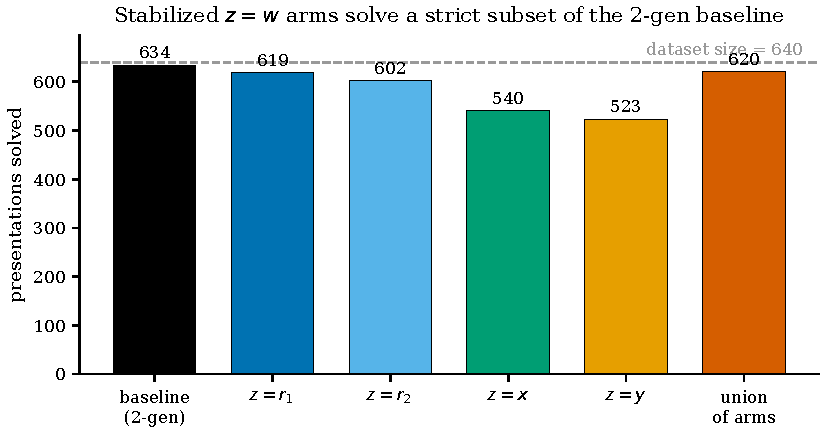
\includegraphics[width=\textwidth]{arms_bar}
  \caption{Solved counts per arm}\label{fig:arms-a}
\end{subfigure}\hfill
\begin{subfigure}{0.48\textwidth}
  \centering
  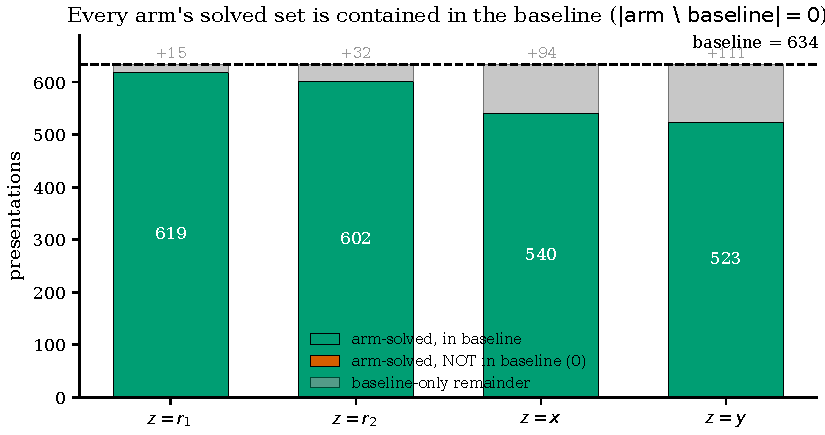
\includegraphics[width=\textwidth]{arms_subset}
  \caption{Containment of solved sets}\label{fig:arms-b}
\end{subfigure}
\caption{Naive $z=w$ stabilization over the $640$ known-solvable MS(1190) presentations at
$5\times10^5$ nodes. (a) Solved counts per arm --- baseline $634$, $r_1\,619$, $r_2\,602$,
$x\,540$, $y\,523$ --- all below the baseline. (b) Containment: every arm's solved set is a
strict subset of the baseline's ($|\text{arm}\setminus\text{baseline}|=0$ for all four
arms; union $620$, intersection $523$), so stabilization reproduces but never extends the
baseline within budget.}
\label{fig:arms}
\end{figure}

\begin{table}[tbp]
\centering
\caption{Naive $z=w$ stabilization over the $640$ known-solvable MS(1190) presentations at
$5\times10^5$ nodes. Every arm's solved set is a strict subset of the baseline's; node and
path-length statistics are computed over solved presentations only.}
\label{tab:arms}
\small
\setlength{\tabcolsep}{3pt}%
\begin{tabular}{lrrrrrc}
\toprule
Arm & Solved/640 & Exhausted & Nodes (median) & Nodes (mean) & Path len (median) & $\subseteq$ baseline? \\
\midrule
baseline & 634 & 6 & 11 & 1662.0 & 8 & --- \\
r1 & 619 & 21 & 13 & 2802.6 & 12 & yes \\
r2 & 602 & 38 & 13 & 3637.1 & 11 & yes \\
x & 540 & 100 & 10 & 14680.7 & 9 & yes \\
y & 523 & 117 & 10 & 21832.7 & 9 & yes \\
\bottomrule
\end{tabular}

\vspace{2pt}
{\footnotesize
$\subseteq$ baseline? tests whether the arm's solved-idx set is a subset of the baseline's solved-idx set, computed directly from the 640-row calibration streams (not assumed).\par
Nodes/Path-len statistics are computed over SOLVED presentations only (budget-exhausted rows report nodes\_explored == budget\_nodes, which would otherwise dominate the mean).\par
}

\end{table}

\subsection{A literature-grounded word bank fails on AK(3)}

We throw the full $97$-word bank (Table~\ref{tab:wordbank}) at both AK(3) forms --- the
textbook presentation and the dataset-representative form --- at $10^5$ and $10^6$ nodes:
$388$ runs ($97\times2\times2$), $0$ solved (Figure~\ref{fig:ak3_plateau}, appendix). At
$10^6$ nodes the minimum-total-length distribution concentrates hard on the floor: the
representative form gives $\{13\!:\!88,\ 14\!:\!2,\ 15\!:\!7\}$ and the textbook form
$\{13\!:\!86,\ 14\!:\!2,\ 15\!:\!9\}$, against a trivial target of total length $3$. Even
the provably-isolatable theory words --- the $w_k$ isolation family of Theorems 6 and
7~\cite{shehper2024hard} --- burn the full $10^6$-node budget and stall on the floor. The
AK(3) floor is $13$ with a small $14$--$15$ tail, and no family, theory-grounded or
brute-force, escapes it within the searched budgets.

\subsection{On solvable targets, only relator-derived words solve --- and only tie the control}

AK(3) returns a $0$-everywhere signal, which alone cannot separate ``no word helps'' from
``no method could help.'' We therefore repeat the identical protocol on two MS presentations
the $2$-generator baseline \emph{does} solve, but only after tens of thousands of nodes
(Figure~\ref{fig:hard_ties}, appendix). On index $625$, $4$ of $98$ words solve: the two
controls $z=r_1$ ($77{,}395$ nodes) and $z=r_2$ ($80{,}111$), plus two \texttt{relhalf}
words derived from $r_1$ and $r_2$ that match those node counts \emph{exactly} ($77{,}395$
and $80{,}111$) --- the same searches in disguise. On index $610$, $2$ of $99$ solve: $z=r_1$
and its \texttt{relhalf} twin, both at $61{,}082$ nodes. Across the ${\sim}180$
generic-family (word $\times$ target) runs, $0$ solve, and the unsolved runs floor at total
length $16$--$25$. No literature-grounded word beats --- or even differs from --- the target's
own relators; greedy substitution does not exploit a named change of variables.

\subsection{Five lanes, zero solves out of 16,870 attempts}

Five attack lanes layer stable-AC structure onto the base search (Table~\ref{tab:lanes},
Figure~\ref{fig:campaign_floor}). The consolidated campaign archive harvests $180{,}645$
distinct Lemma-11 quotients --- each stably AC-equivalent to AK(3) by construction of the
harvest pipeline, verified end-to-end on the exported certificates, and none previously
searched, since they exist only after a stabilize--substitute--eliminate chain --- and runs
$16{,}870$ solve attempts over $6{,}058$ distinct candidates: $0$ of $16{,}870$ attempts
solved. The campaign floor histogram is $\{13\!:\!16{,}844,\ 19\!:\!23,\ 20\!:\!3\}$. Lane
A (meet-in-the-middle: $2$ probes at $2\times10^6$ nodes/side against $1{,}177$
symmetry-expanded targets) records $0$ hits and was deprioritized once all $151$ in-cap
catalog leaves proved plain-AC-trivial. Lane B ($6$ stable-move-search probes,
$3\times10^5$--$8\times10^5$ nodes) solves none; its positive controls confirm the machinery
is sound --- known-easy instances trivialize \emph{through} the stabilize/eliminate moves (a
corrected-family instance in $3$ steps, two MS instances in $1$; Table~\ref{tab:certs}) ---
so the $0/6$ on the hard probes is a search miss, not a plumbing failure. Lane C
(trivial-$z$ stabilization) floors at total length $14$, $15$, $16$ for $n=3,4,5$ --- exactly
one added unit of floor per contentless generator. Lane E is \S4.6. A fully local
reproduction --- $1{,}937$ solve attempts over a $1{,}006$-candidate census --- bottoms out at
exactly $13$ on every one. One coincidence deserves a line: the trivial target is total
length $3$ for a $3$-generator state and $2$ for a $2$-generator state, yet both the
$3$-generator stabilized searches and the $2$-generator quotient searches floor at the same
total length $13$.

\begin{table}[tbp]
\centering
\caption{Five attack lanes layering stable-AC structure on the base search: $0$ of
$16{,}870$ Lane-D solve attempts (over $6{,}058$ distinct candidates from $180{,}645$
harvested quotients) and $0$ of the $14$ grid probes (Lanes A--C) succeed, all flooring
within their searched budgets.}
\label{tab:lanes}
\footnotesize
\setlength{\tabcolsep}{3pt}%
\begin{tabular}{@{}p{0.10\textwidth}p{0.35\textwidth}p{0.15\textwidth}p{0.08\textwidth}p{0.24\textwidth}@{}}
\toprule
Lane & Method & Trials/Probes & Solved & Floor reached \\
\midrule
A: MITM & Meet-in-the-middle ball search from AK(3)/P25 (targets = 1,177 certified stably-trivial states) & 2 @ 2,000,000 nodes/side & 0/2 & 13 \\
B: StableSolver & Best-first search over substitution + stabilize + eliminate moves & 6 @ 300k-800k nodes & 0/6 & 13 \\
C: trivial-z & n-generator (n=3,4,5) trivial-z stabilization + plain greedy substitution, rep \& textbook forms & 6 @ 800k-2,000,000 nodes & 0/6 & 14-16 (rep\_n3=14, rep\_n4=15, rep\_n5=16, textbook\_n3=14, textbook\_n4=15, textbook\_n5=16) \\
D: plateau-elim & Harvest visited stabilized states, Lemma-11 eliminate, dedupe by signed-relabel symmetry, greedy re-solve every fresh 2-gen quotient & 16,870 trials / 6,058 distinct (180,645 harvested) & 0/16,870 & 13:16,844; 19:23; 20:3 \\
E: RL beam & Beam search with a pretrained 2-generator PPO policy (zero-shot), widths 512 and 2048 & 155 + 30 & 0/155 + 0/30 & n/a (beam search records no min-total-length floor) \\
\bottomrule
\end{tabular}

\vspace{2pt}
{\footnotesize
Trials/Solved/floor counts for lanes A-D are computed directly from archive/campaign\_grid\_probes.jsonl.gz (A, B, C) and archive/campaign\_trials.jsonl.gz (D), cross-checked against collect\_summary.json's authoritative totals (trials=16870, candidates=180645, grid\_probes=14); all matched.\par
Lane D's source-facet breakdown (trial counts): laneD:D1=5866, laneD:D2=5350, laneD:D3=5497, resolve=157.\par
Lane E counts are row counts of runs/beam\_laneD\_floor.csv (155) and runs/beam\_laneD\_floor\_w2048.csv (30); both have solved=False on every row.\par
}

\end{table}

\begin{figure}[tbp]
\centering
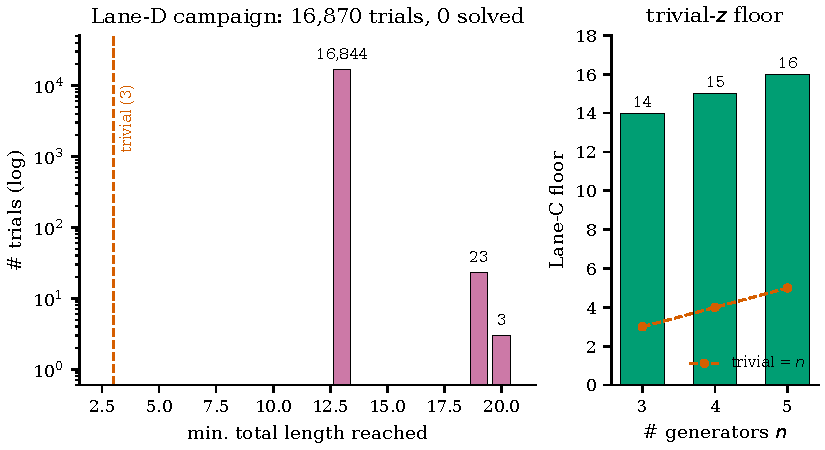
\includegraphics[width=\textwidth]{campaign_floor}
\caption{Floor histogram across the consolidated five-lane campaign: $16{,}870$ solve
attempts over $6{,}058$ distinct candidates (from $180{,}645$ harvested Lemma-11
quotients), $0$ solved, with floors $\{13\!:\!16{,}844,\ 19\!:\!23,\ 20\!:\!3\}$. The
trivial-$z$ control (Lane C) adds one unit of floor per contentless generator ($14/15/16$
for $n=3/4/5$).}
\label{fig:campaign_floor}
\end{figure}

\subsection{Zero-shot policy transfer fails on floor states}

We probe whether a learned policy escapes where greedy stalls (Figure~\ref{fig:rl_gap},
appendix). A pretrained $2$-generator PPO policy with beam search from prior
work~\cite{fagan2026twohump}, run zero-shot at beam width $512$, solves $0$ of $155$ floor
states, while the \emph{same} system solves $155/155$ of its own training-distribution
items (mean path length $6.1$, max $16$). Escalating to beam width $2048$ with temperature
annealing on the hardest $30$-state core still solves $0$. This is strictly an
out-of-distribution transfer probe of a fixed policy, not a statement about reinforcement
learning in principle: the gap between $155/155$ in-distribution and $0/155$ on the floor
is an OOD gap, not an RL ceiling.

\subsection{The cap is not the binding constraint}

If the per-relator cap $L=24$ were the wall, relaxing it should convert failures into
solves; it does not (Figure~\ref{fig:cap_hump}, Appendix~\ref{app:cap}). Raising $L$ from
$24$ to $48$ leaves the search's visited set \emph{byte-identical} in $16$ of $16$ (form
$\times$ hero-word) runs at $10^5$ nodes --- the search never wants a longer relator at these
budgets. Harvesting with the caps raised ($l_{\text{cap}}=48$, total-length cap $40$)
produces $250{,}397$ unique candidates, of which $212{,}913$ lie in the previously
unreachable $>24$ region; a stratified sample of $1{,}800$ ($100$ per length bucket
$25$--$40$ plus $200$ short controls) solved at maximum length $60$ yields $0$ of $1{,}800$
attempts solved, with every single one flooring at exactly total length $13$. Within the
tested range the cap is not the binding constraint ($L\le48$, solve cap $60$): the floor is
a property of the region, not of the fence around it.

\begin{figure}[tbp]
\centering
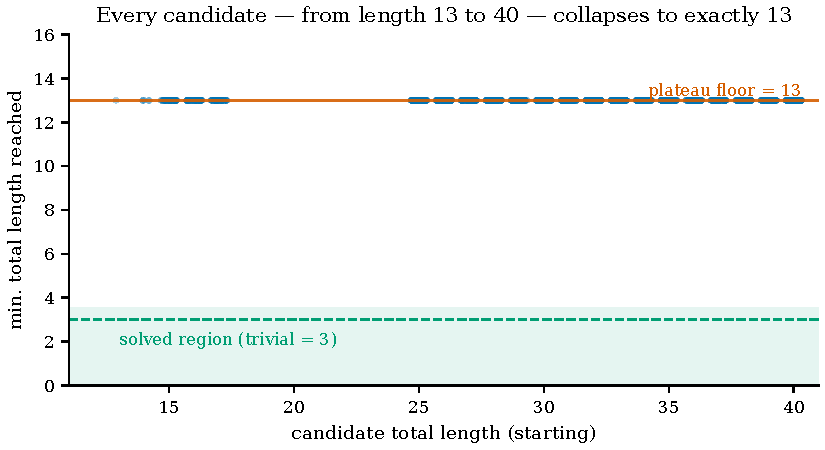
\includegraphics[width=\textwidth]{cap_hump}
\caption{The per-relator cap is not the binding constraint in the tested range. Raising $L$
from $24$ to $48$ leaves the visited set byte-identical in $16/16$ runs at $10^5$ nodes; a
stratified sample of $1{,}800$ candidates ($212{,}913$ of $250{,}397$ raised-cap candidates
lie in the previously unreachable $>24$ region) solved at maximum length $60$ gives $0$
solved, every one flooring at exactly total length $13$.}
\label{fig:cap_hump}
\end{figure}

\subsection{The floor has exactly two canonical representatives}

A floor census over the $1{,}006$ local candidates settles \emph{where} the search funnels.
Every candidate lands on one of exactly two canonical (signed-relabel) representatives of
the length-$13$ floor of AK(3)'s AC-class (Figure~\ref{fig:two_floors},
Tables~\ref{tab:certs}, \ref{tab:floorcensus}): $F=\langle x,y \mid y^{-2}xyx^{-2},\
y^{-3}x^{-2}yx\rangle$, hit $712$ times ($70.8\%$), and AK(3)'s own reduced form, hit $294$
times ($29.2\%$). A $21$-move substitution path $F\to\mathrm{AK}(3)$ was extracted and
certified, passing both the engine author's verifier and the independently authored one
(Table~\ref{tab:certs}). The accessible region therefore funnels onto a \emph{single}
AC-class floor with two canonical representatives; $F$ --- the dominant attractor, reached
$2.4\times$ more often than AK(3) itself --- is a $2$-generator presentation AC-equivalent to
AK(3) that, to the authors' knowledge, has not previously appeared as a search seed. The
structural obstruction is now visible: the certified Appendix-F path peaks at total length
$25$, i.e. $12$ above the floor, so escaping the floor requires climbing --- precisely what
length-ordered search structurally resists.

\begin{figure}[tbp]
\centering
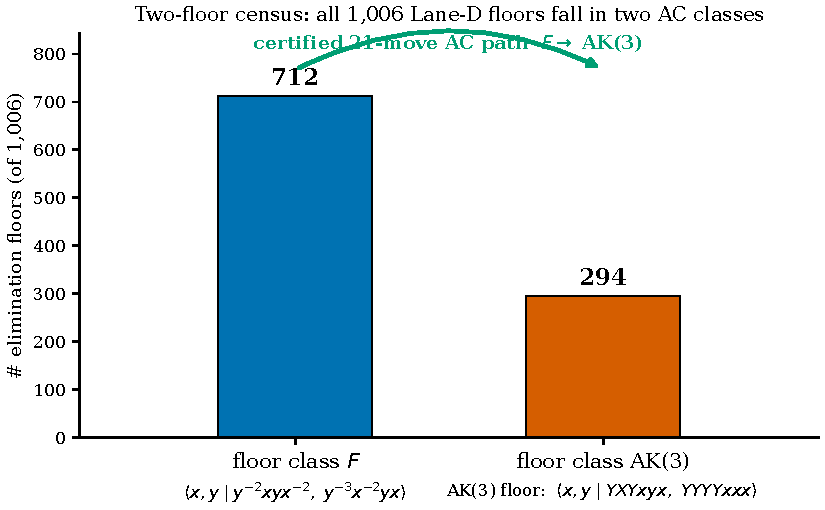
\includegraphics[width=\textwidth]{two_floors}
\caption{The length-$13$ floor of AK(3)'s AC-class has exactly two canonical
(signed-relabel) representatives, over the $1{,}006$-candidate local census: $F=\langle x,y
\mid y^{-2}xyx^{-2},\ y^{-3}x^{-2}yx\rangle$ ($712$, $70.8\%$; reached $2.4\times$ more
often than AK(3)) and AK(3)'s own reduced form ($294$, $29.2\%$), joined by a certified
$21$-move substitution path $F\to\mathrm{AK}(3)$ that peaks at total length $25$, i.e. $12$
above the floor.}
\label{fig:two_floors}
\end{figure}

\begin{table}[tbp]
\centering
\caption{The length-$13$ floor of AK(3)'s AC-class has exactly two canonical
(signed-relabel) representatives over the $1{,}006$-candidate census: $F$ (the dominant
attractor, Class~1) and AK(3)'s own reduced form (Class~2).}
\label{tab:floorcensus}
\small
\begin{tabular}{lrrl}
\toprule
Floor class & Count & Share & Relators \\
\midrule
Class 1 (= laneF's F) & 712 & 70.8\% & YYxyXX, YYYXXyx \\
Class 2 (= AK(3)) & 294 & 29.2\% & YXYxyx, YYYxxxx \\
\bottomrule
\end{tabular}

\vspace{2pt}
{\footnotesize
Floor class = the greedy search's canonical terminal state (floor\_mkey, min over signed relabelings) after re-solving every merged Lane-D quotient at a 25,000-node budget; all 1,006 probes bottom out at total relator length 13 in exactly 2 distinct classes.\par
Relator words translate the int-array floor\_state (1=x, -1=X, 2=y, -2=Y).\par
Identity check (mitm.symmetry\_keys, live): the majority class's floor state is the laneF\_F\_to\_AK3 cert's F start state (mod signed relabeling); the minority class's floor state is AK(3) itself (mod signed relabeling).\par
}

\end{table}

\input{sections/05_limitations}
\section{Conclusion and Next Steps}\label{sec:conclusion}

AK(3)'s stable AC-triviality remains open: the premise that had appeared to settle it was
independently re-verified as rescinded in prior work \cite{shehper2024hard}. Within the
searched budgets ($\leq 2\times10^6$ nodes per run, beam width $\leq 2048$), stabilizing AK(3)
in every tested form adds nothing over plain 2-generator greedy substitution --- naive $z=w$
arms solve strict subsets of what the unstabilized baseline already solves, no word in the
97-word bank beats a target's own relators as a stabilizer, and across five
differently-shaped search lanes, 0 of 16,870 attempts solved. The relator-length cap does
not bind in the tested range ($L\leq48$, solve cap 60): raising it changes nothing. And the
entire accessible region funnels onto a length-13 floor with exactly two canonical
(signed-relabel) representatives of that floor --- $F$, a 2-generator presentation
AC-equivalent to AK(3) (71\% of the census), and AK(3)'s own reduced form (29\%) --- joined by
a certified 21-move AC path (\ref{fig:two_floors}). That two-floor result, not a solve, is
this paper's certified structural contribution: a new fact about AK(3)'s neighborhood,
established independently of whether AK(3) itself ever trivializes.

The negative and the floor structure point at the same mechanism. Greedy substitution,
ordered by shrinking total length, cannot assemble a Lemma-11 change-of-variables one
length-decreasing move at a time, because the cancellation the lemma provides is inherently
a batch effect, not a gradual descent --- the useful move is an atomic destabilization
supermove, not incremental substitution. The literature's own 53-move trivialization path
confirms this directly: it peaks at total length 25 before falling to trivial, climbing
before it descends. Read this way, the two-hump landscape reported for the unstable problem
\cite{fagan2026twohump} reappears here one level up --- a second hump, for the stable problem,
separating the length-13 floor from the trivial presentation, that only a search capable of
climbing (not just shrinking) has any chance of crossing.

\paragraph{Next steps.}
\begin{enumerate}
  \item Make Lemma-11 elimination itself a first-class, length-increasing search move,
    gated against the certified 21-move chain; the StableSolver machinery already exists
    (\ref{sec:methods}) and needs scaling, not redesign.
  \item Attack $F$ directly. It is the dominant floor representative (71\% of the census)
    and, unlike AK(3), was never itself used as a search seed before this work; inverting
    the certified $F\to$AK(3) bridge gives a ready-made route to search outward from it.
  \item Train or fine-tune the RL policy on floor quotients and stabilized states directly,
    closing the zero-shot out-of-distribution gap noted in \S5.
  \item Escalate the archived 180,645-quotient candidate pool at 10--40$\times$ the tested
    budgets; its deduplicated, resumable construction (\ref{app:repro}) makes this a scaling
    exercise, not a rerun from scratch.
  \item Test non-length-ordered or globally-guided search; the Appendix-F path's length-25
    peak is a concrete target phenomenon that a length-ordered search cannot produce by
    construction.
  \item Build a per-presentation word-bank generator that generalizes the
    target-derived-relator construction used for the hard-target controls, so word choice no
    longer depends on AK($n$)-specific theory.
  \item Export certificates for the remaining 137 catalog-leaf classifications and extend
    the independent verifier to cover the harvest pipeline end to end, not only the
    certificates already exported.
\end{enumerate}

Negative results of this breadth, reproducible and certificate-grade, carve the search
space for anyone who takes up this problem next. The floor census, the certificate chains,
and the deduplicated candidate archive are released, on acceptance, as a foundation for
exactly that.


\bibliographystyle{plainnat}
\bibliography{refs}

\newpage
\appendix

\input{sections/A_glossary}
\section{The acx-cert-v1 Certificate Schema and Its Verification}\label{app:certs}

Every solution and every stable-AC equivalence claimed in this paper is exported as an
acx-cert-v1 JSON certificate and checked by two independently written verifiers before it
is reported.

\subsection{Schema}

A certificate is a JSON object with fields: \texttt{certificate\_version} (schema version
string); \texttt{name}; \texttt{claim} (a human-readable statement of what is being
certified); \texttt{start} and \texttt{end} (each an object \texttt{\{n\_gen, relators\}});
\texttt{end\_is\_trivial} (boolean, true iff \texttt{end} must equal the trivial
presentation on \texttt{n\_gen} generators); \texttt{steps} (an ordered list of length
$T$); \texttt{states} (the list of intermediate presentations, length $T+1$, with
\texttt{states[0]==start} and \texttt{states[-1]==end}); and \texttt{meta} (free-form
provenance --- source paper or line numbers, generator naming, and similar bookkeeping).

\subsection{Step types}

Six step types are implemented; the field names below are exact, not paraphrased:

\begin{itemize}
  \item \textbf{concat} \texttt{\{i, j, sign\}} --- $r_i \to$ freely-reduced$(r_i \cdot
    r_j^{\text{sign}})$ (AC1; \texttt{sign=-1} concatenates with $r_j^{-1}$).
  \item \textbf{conjugate} \texttt{\{i, g\}} --- $r_i \to$ freely-reduced$(g\cdot r_i\cdot
    g^{-1})$ (AC3).
  \item \textbf{stabilize} \texttt{\{z, w\}} --- appends generator $z=$ \texttt{n\_gen}$+1$
    and the cyclically-reduced relator $z\cdot w^{-1}$ (AC4 plus realizing $z=w$).
  \item \textbf{eliminate} \texttt{\{gen, ri, ...\}} --- Lemma-11 removal of \texttt{gen}
    using its exactly-once occurrence in relator \texttt{ri}; generators above \texttt{gen}
    are renumbered down by one (the packaged AC5).
  \item \textbf{relabel} \texttt{\{perm, invert\}} --- a bijective, sign-respecting
    permutation of the generator set: an AC-equivariant renaming, not a move on relators.
  \item \textbf{substitution} \texttt{\{ci, a, b, i, j, c\_inv\}} --- the composite move used
    by the base greedy solver (\ref{sec:methods}); verified by checking that the resulting
    state lies in the recomputed neighbor set of the preceding state, rather than by
    replaying finer sub-steps.
\end{itemize}

There is no separate step type for a bare AC2 inversion of a whole relator. A full-relator
sign flip is instead absorbed by the canonical-equality quotient the verifiers already
apply (reorder relators, cyclically rotate, invert) --- see the mutation-sensitivity note
below, where this distinction mattered in practice.

\subsection{Verification levels}

\begin{itemize}
  \item \textbf{L1 (replay).} Recompute each step's post-state from its recorded parameters
    and the preceding state; it must equal the next recorded state exactly.
  \item \textbf{L2 (preconditions).} \texttt{eliminate}'s generator must occur exactly once
    in the cited relator; \texttt{relabel}'s permutation must be bijective and
    sign-consistent; every letter must lie in the valid signed-generator range for that
    state's \texttt{n\_gen}.
  \item \textbf{L3 (global invariants).} Every state must be balanced (\texttt{n\_gen}
    equal to the relator count, no empty relator); the abelianization matrix's determinant
    must have absolute value $1$ at every state, computed by exact-integer Bareiss
    elimination (no floating point); if \texttt{end\_is\_trivial} is claimed, the end state
    must equal $\langle x_1,\dots,x_k\mid x_1,\dots,x_k\rangle$ up to relator reordering.
\end{itemize}

\subsection{Two independent verifiers}

Every certificate is checked by the engine author's verifier and by a second verifier
authored black-box from the schema and the math above alone, with no access to the engine's
source and its own free/cyclic reduction, canonicalization, integer-determinant, and
step-replay logic. Across the campaign the two verifiers together performed $20{,}947$
checks with $0$ failures. All five exported chain certificates pass both
(Table~\ref{tab:certs}): \texttt{appendixF\_P25\_to\_AK3} (53 steps, the literature's
$\mathrm{P25}\to\mathrm{AK}(3)$ replay of \ref{app:misprint}), \texttt{laneF\_F\_to\_AK3}
(21 steps, the path from $F$ --- a 2-generator presentation AC-equivalent to AK(3) --- to AK(3)
itself), and three small stable-solver certificates recording in-search destabilizations
(3, 1, and 1 steps respectively).

\begin{table}[tbp]
\centering
\caption{The five exported acx-cert-v1 chain certificates, each passing both the engine
author's verifier and the independently authored black-box verifier.}
\label{tab:certs}
\small
\setlength{\tabcolsep}{3pt}%
\begin{tabular}{@{}p{0.27\textwidth}p{0.55\textwidth}rr@{}}
\toprule
Certificate & Claim & Steps & States \\
\midrule
appendixF\_P25\_to\_AK3 & P25 is AC-equivalent to AK(3) via the 53 printed Appendix-F h-moves (arXiv:2408.15332v2). & 53 & 54 \\
laneB\_M3corr\_hero8\_500 & Stable-AC trivialization of M3corr\_hero8 found by StableSolver. & 3 & 4 \\
laneB\_ms0 & Stable-AC trivialization of ms0\_plain found by StableSolver. & 1 & 2 \\
laneB\_ms0\_stab & Stable-AC trivialization of ms0\_stab found by StableSolver. & 1 & 2 \\
laneF\_F\_to\_AK3 & F = \textless{}x,y | YYxyXX, YYYXXyx\textgreater{} is plain-AC-equivalent to AK(3) (up to signed relabeling); explicit substitution path found by greedy search. & 21 & 22 \\
\bottomrule
\end{tabular}

\vspace{2pt}
{\footnotesize
All 5 certificates pass both experiments/stable\_ac/ak3\_stable\_proof/verify\_certificate.py and the independently-authored independent\_verifier.py (confirmed live: verify\_certificate.py=True, independent\_verifier.py=True).\par
}

\end{table}

\subsection{Mutation sensitivity}

Sign flips, corrupted target states, swapped intermediate states, and mis-pointed
eliminations are all rejected by both verifiers. One candidate mutation was initially
flagged as accepted; on inspection it was not a soundness hole but a genuinely valid
alternative move --- inverting a relator of length one is itself a legal AC2 move, correctly
treated as a no-op by the canonical-equality quotient rather than as a tamper. A
semantically meaningful tamper test therefore has to flip an \emph{interior} letter of a
relator of length at least three in a middle state, not merely a sign.

\subsection{Coverage and chain composition}

Of the 151 catalog leaves classified during the campaign, 14 have exported,
machine-verified leaf certificates; the remaining 137 classifications are recorded as data
(solved/unsolved, node count, floor reached) but were not individually exported as
certificates. Certificates concatenate whenever one certificate's end state matches the
next certificate's start state exactly, so a full stable-AC chain --- stabilize $\to$
substitution path $\to$ eliminate $\to$ 2-generator trivialization path, further composed
with the P25 bridge of \ref{app:misprint} --- assembles automatically into a single
machine-checkable certificate. This composition machinery already produces every
certificate reported above and would apply unchanged to any future solve.

\section{Extended Data Tables}\label{app:tables}

This appendix collects extended data behind the six numbered tables of the main text
(Tables~\ref{tab:litchecks}--\ref{tab:floorcensus}) and discusses the three figures that
live only in the appendix (\ref{fig:ak3_plateau}, \ref{fig:hard_ties}, \ref{fig:rl_gap}).
Every value below is read from the same digest files that produced the main-text tables and
figures, and is independently re-derivable from the raw record streams (\ref{app:repro}).

\subsection{Extended per-arm statistics}

Table~\ref{tab:arms} reports median nodes and median path length, over solved presentations
only, for the naive $z=w$ stabilization arms. The full min/max/mean/median breakdown, over
the same solved-only convention, is:

\begin{center}
\small
\begin{tabular}{@{}lll@{}}
\toprule
Arm & Nodes (min / max / mean / median) & Path length (min / max / mean / median) \\
\midrule
baseline & 3 / 77,385 / 1,662.0 / 11 & 2 / 710 / 32.6 / 8 \\
$r_1$    & 5 / 239,578 / 2,802.6 / 13 & 4 / 714 / 33.8 / 12 \\
$r_2$    & 4 / 291,479 / 3,637.1 / 13 & 3 / 715 / 29.9 / 11 \\
$x$      & 4 / 326,326 / 14,680.7 / 10 & 3 / 102 / 12.1 / 9 \\
$y$      & 4 / 491,437 / 21,832.7 / 10 & 3 / 102 / 11.5 / 9 \\
\bottomrule
\end{tabular}
\end{center}

The $x$ and $y$ arms' wide gap between median ($10$) and mean ($14{,}680.7$ / $21{,}832.7$)
node counts, set against a comparatively tight path-length distribution (max $102$), is the
alias-orbit effect noted in \ref{sec:results}: defining $z$ by an already-present generator
does not lengthen solutions, it multiplies equivalent detours the search must exhaust
before terminating.

\subsection{The 97-word literature-grounded bank}

Table~\ref{tab:wordbank} gives family sizes. The full bank --- 95 words across seven
families, plus the two per-target control words $z=r_1,r_2$ added at run time to reach 97 ---
grouped by family in escalation-priority order, is:

\begin{itemize}
  \item \textbf{relhalf} (17): \texttt{xyx, yxy, xxx, yyyy, yxx, xxy, xyy, yyx, XYX, YXY,
    XXX, YYYY, xyxY, Yxyx, xx, yy, yyy}
  \item \textbf{wk} (17): \texttt{yyyyyyyyXyxy, yyyyyyyXyxy, yyyyyyXyxy, yyyyyXyxy,
    yyyyXyxy, yyyXyxy, yyXyxy, yXyxy, Xyxy, YXyxy, YYXyxy, YYYXyxy, YYYYXyxy, YYYYYXyxy,
    YYYYYYXyxy, YYYYYYYXyxy, YYYYYYYYXyxy}
  \item \textbf{wstar} (5): \texttt{YxyX, XyxY, xYXy, yXYx, xYxY}
  \item \textbf{conj} (14): \texttt{x, xyX, yxY, y, Xyx, Yxy, xyxYX, yxyXY, xYxyX, YxyXy,
    xxyXX, yyxYY, XYxyx, XyxYx}
  \item \textbf{comm} (6): \texttt{XYxy, YXyx, xyXY, yxYX, XyXy, xyXYX}
  \item \textbf{ms} (3): \texttt{Xyxyy, yxyx, xyxyy}
  \item \textbf{brute} (33): \texttt{X, Y, xy, xY, XX, Xy, XY, yx, yX, Yx, YX, YY, xxY, xYx,
    xYX, xYY, XXy, XXY, XyX, Xyy, XYx, XYY, yXX, yXy, yXY, yyX, Yxx, YxY, YXX, YXy, YYx, YYX,
    YYY}
\end{itemize}

Each name is the induced word $w$ in $x^{\pm1},y^{\pm1}$ under the encoding of
\ref{app:glossary} (capital letter = inverse); each induces a $z$-relator $z\cdot w^{-1}$,
deduplicated by that induced relator and dropped if it violates the per-relator cap $L=24$.

\subsection{Campaign facet breakdown}

Lane D's $16{,}870$ solve attempts (Table~\ref{tab:lanes}) are drawn from four resumable
facets, every one contributing $0$ solved: D1 ($5{,}866$ solve attempts), D2 ($5{,}350$),
D3 ($5{,}497$), and a resolve pass at the raised per-relator cap $L=40$ ($157$ solve
attempts, probing whether the $L=24$ cap specifically --- as opposed to the total-length cap
--- was pruning a viable descent among the shortest candidates). The four facets sum to the
reported $16{,}870$; $0$ of $16{,}870$ solve attempts succeed across all four.

\subsection{Floor census detail}

The two canonical (signed-relabel) representatives of the length-13 floor of AK(3)'s
AC-class (Table~\ref{tab:floorcensus}) have relators, under the encoding $x\!\to\!1,\
X\!\to\!-1,\ y\!\to\!2,\ Y\!\to\!-2$:

\begin{itemize}
  \item $F$ --- a 2-generator presentation AC-equivalent to AK(3): \texttt{YYxyXX} /
    \texttt{YYYXXyx}, i.e. $y^{-2}xyx^{-2}$ and $y^{-3}x^{-2}yx$ --- the dominant attractor,
    $712/1006$ ($70.8\%$).
  \item AK(3)'s own reduced form: \texttt{YXYxyx} / \texttt{YYYxxxx} --- $294/1006$
    ($29.2\%$).
\end{itemize}

Each census candidate is assigned by canonicalizing its terminal state and checking
equality with one of these two representatives up to signed relabeling (\ref{app:glossary});
no third representative appears anywhere in the 1,006-candidate census.

\subsection{Grid-probe list}

Beyond Lane D's harvested-quotient attempts, the campaign ran $14$ additional grid probes
(Table~\ref{tab:lanes}, Lanes A--C):

\begin{center}
\small
\begin{tabular}{@{}l p{0.36\textwidth} l l@{}}
\toprule
Lane & Probe & Nodes & Floor \\
\midrule
A (MITM) & from AK(3), against 1,177 targets & 2,000,000 & 13 \\
A (MITM) & from P25, against 1,177 targets & 2,000,000 & 13 \\
B (StableSolver) & hero-8 bank, $g\le3$, gen-penalty 2, from P25 & 800,000 & 13 \\
B (StableSolver) & hero-8 bank, $g\le3$, gen-penalty 2, from AK(3) & 800,000 & 13 \\
B (StableSolver) & hero-8 bank, $g\le3$, gen-penalty 1, from AK(3) & 800,000 & 13 \\
B (StableSolver) & hero-8 bank, $g\le4$, gen-penalty 2, from AK(3) & 800,000 & 13 \\
B (StableSolver) & full 95-word bank, $g\le3$, from AK(3) & 300,000 & 13 \\
B (StableSolver) & full 95-word bank, $g\le3$, from P25 & 300,000 & 13 \\
C (trivial-$z$) & rep form, $n=3$ & 1,500,000 & 14 \\
C (trivial-$z$) & textbook form, $n=3$ & 2,000,000 & 14 \\
C (trivial-$z$) & rep form, $n=4$ & 1,000,000 & 15 \\
C (trivial-$z$) & textbook form, $n=4$ & 1,500,000 & 15 \\
C (trivial-$z$) & rep form, $n=5$ & 800,000 & 16 \\
C (trivial-$z$) & textbook form, $n=5$ & 1,000,000 & 16 \\
\bottomrule
\end{tabular}
\end{center}

All 14 probes floor within their searched budgets; $0$ of 14 solve.

\subsection{Discussion of the appendix figures}

\begin{figure}[tbp]
\centering
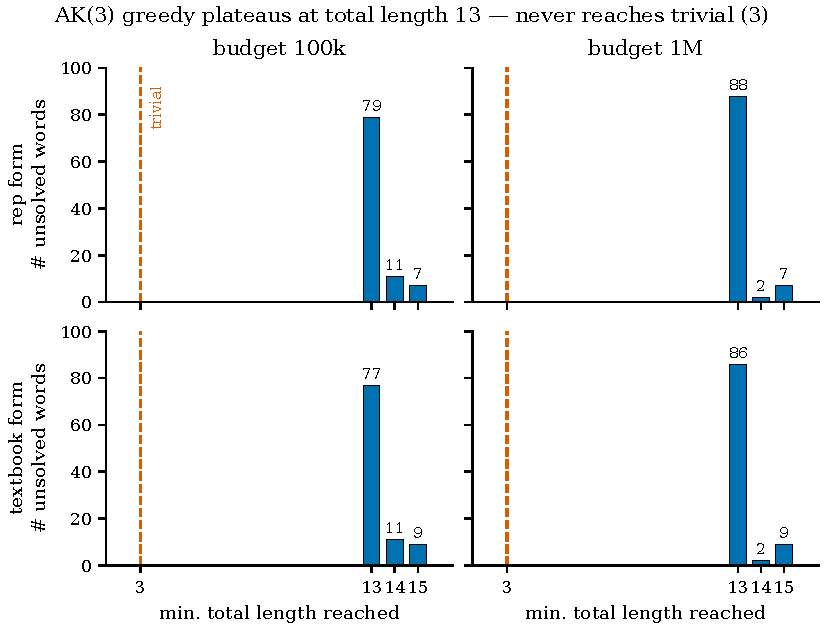
\includegraphics[width=\textwidth]{ak3_plateau}
\caption{Minimum-total-length reached by the $97$-word bank on both AK(3) forms (trivial
target $=3$); $0$ of $388$ solve attempts succeed. At $10^6$ nodes the distribution
concentrates on the floor --- representative form $\{13\!:\!88,14\!:\!2,15\!:\!7\}$, textbook
form $\{13\!:\!86,14\!:\!2,15\!:\!9\}$ --- a floor of $13$ with a small $14$--$15$ tail that
even the provably-isolatable $w_k$ theory words do not escape.}
\label{fig:ak3_plateau}
\end{figure}

\textbf{Figure~\ref{fig:ak3_plateau}.} At $10^5$ nodes the representative form's floor
histogram is already concentrated ($79$ words at floor $13$, $11$ at $14$, $7$ at $15$);
escalating every unsolved word tenfold to $10^6$ nodes tightens the concentration further
($88/2/7$) rather than dislodging any word past the floor, and the textbook form shows the
identical pattern ($77/11/9$ at $10^5$, sharpening to $86/2/9$ at $10^6$). Every one of the
$97\times2\times2=388$ solve attempts across both forms and both budgets records $0$ solved,
within the searched budgets, against a trivial target of total length $3$; more nodes
concentrate the distribution on the floor rather than escaping it, evidence that the
obstruction is structural rather than a matter of search depth.

\begin{figure}[tbp]
\centering
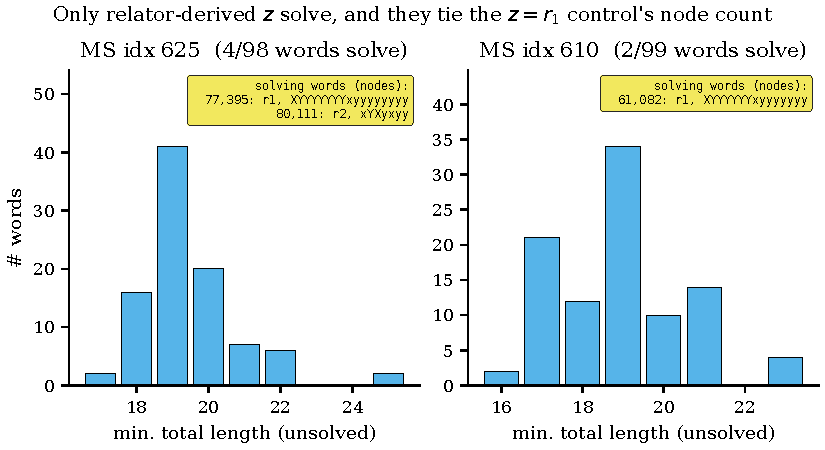
\includegraphics[width=\textwidth]{hard_ties}
\caption{Word-bank protocol on two hard-but-solvable MS targets. Index $625$: $4$ of $98$
words solve --- controls $z=r_1$ ($77{,}395$ nodes) and $z=r_2$ ($80{,}111$) plus two
relator-derived \texttt{relhalf} words tying those exact node counts. Index $610$: $2$ of
$99$ solve ($z=r_1$ and its \texttt{relhalf} twin, both $61{,}082$). All ${\sim}180$
generic-family runs fail (floor $16$--$25$); no clever word beats or even differs from the
target's own relators.}
\label{fig:hard_ties}
\end{figure}

\textbf{Figure~\ref{fig:hard_ties}.} On the two hard-but-solvable controls, the floor
histograms sit far above AK(3)'s own (index $625$: range $17$--$25$, peaking at $19$ with
$41$ of $98$ words; index $610$: range $16$--$23$, peaking at $19$ with $34$ of $99$ words),
confirming these are genuinely different, easier landscapes with their own internal spread.
Yet the only words that solve are, in both cases, exactly the target's own relators and
their relator-derived \texttt{relhalf} twins, and they solve at identical node counts (index
$625$: $r_1$ and its \texttt{relhalf} twin both at $77{,}395$ nodes; $r_2$ and its twin both
at $80{,}111$; index $610$: $r_1$ and its twin both at $61{,}082$) --- the same search in
disguise, not a shortcut. Within the searched $10^5$-node screen (the specified $10^6$-node
full tier was not run on these generic-family words), no structurally distinct word ever
solves either target.

\begin{figure}[tbp]
\centering
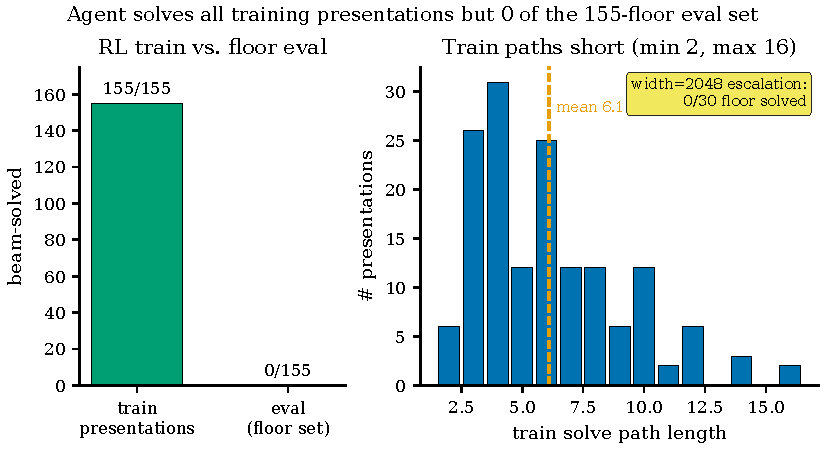
\includegraphics[width=\textwidth]{rl_gap}
\caption{Zero-shot out-of-distribution transfer of a pretrained $2$-generator PPO+beam
policy. It solves $155/155$ of its own training-distribution items (mean path $6.1$, max
$16$) but $0$ of $155$ floor states at beam width $512$; escalation to beam width $2048$
with temperature annealing still solves $0$ of the hardest $30$. The gap is an OOD gap, not
an RL ceiling.}
\label{fig:rl_gap}
\end{figure}

\textbf{Figure~\ref{fig:rl_gap}.} The pretrained policy's own training-distribution path
lengths are short and tightly clustered (mean $6.1$, range $2$--$16$, mode at length $4$:
$31$ of $155$ items), and it solves all $155$ of $155$ solve attempts on that distribution.
Run zero-shot on the $155$ floor and stabilized states at beam width $512$, $0$ of $155$
solve attempts succeed; widening to beam width $2048$ with temperature annealing on the
hardest $30$-state core, $0$ of $30$ solve attempts succeed. Within these two beam-search
configurations, the size of this gap --- perfect in-distribution, zero out-of-distribution,
on states sharing the same 2-generator alphabet the policy was trained on --- is the sharpest
illustration in the campaign that the floor resists every method family tried, learned or
hand-designed, within the budgets searched.

\section{Reproducibility and Artifact Details}\label{app:repro}

\subsection{Data and artifacts}

\begin{itemize}
  \item \textbf{MS(1190) dataset.} The $640$-presentation known-solvable prefix used
    throughout \ref{sec:methods}, drawn from the Miller--Schupp benchmark
    \cite{miller1999ms}.
  \item \textbf{Consolidated candidate/trial archives.} JSONL.gz streams with one record
    per (presentation, arm/word/candidate, budget) triple and full per-record provenance ---
    source form, generator and relator words, node count, floor reached, solved flag.
  \item \textbf{Certificates.} JSON, schema of \ref{app:certs}.
\end{itemize}

All of the above, together with the two acx-cert-v1 verifiers, are released on acceptance.
The source MS(1190)/AC-benchmark datasets this campaign builds on are released under a data
license (CC BY 4.0) by \cite{fagan2026twohump}; the campaign's own derived artifacts --- word
bank, quotient archive, certificates --- will be released under the same terms.

\subsection{Per-campaign recipe}

Six campaigns, each an independent, resumable, append-only JSONL stream keyed by (dataset,
idx-or-form, word-or-arm, budget):

\begin{enumerate}
  \item \textbf{Baseline reproduction} (cap-semantics check, \ref{sec:methods}). Entry:
    \texttt{run\_greedy.py}. Parameters: \texttt{--cap \{sum,per\_relator\} --budget
    \{1e5,1e6\} --workers N}. Output: one stream per (cap, budget) tier, one record per
    presentation index, distinguishing the per-relator cap ($L=24$) from the original sum
    cap.
  \item \textbf{Naive $z=w$ arms} (Table~\ref{tab:arms}). Entry:
    \texttt{run\_greedy\_sweep.py}. Parameters: arm $\in\{$baseline$,r_1,r_2,x,y\}$, budget
    $5\times10^5$, two-phase light/heavy worker scheduling so cheap instances finish first
    and memory-heavy ones run at low parallelism. Output: one stream per arm, records keyed
    by (dataset, idx, arm, budget) so arms merge directly for the subset/union comparison
    of \ref{sec:results}.
  \item \textbf{AK(3) word bank} (Table~\ref{tab:wordbank}). Entry:
    \texttt{run\_ak3\_wormhole.py}. Parameters: form $\in\{$textbook, rep$\}$, the 97-word
    bank, a two-tier budget ($10^5$-node screen, escalate every unsolved word to $10^6$),
    per-relator cap $L=24$. Output: one stream per (form, budget), named by the pattern
    \texttt{ak3\_<form>\_<budget>.jsonl}, keyed by word name.
  \item \textbf{Hard-target controls} (Figure~\ref{fig:hard_ties}). Entry:
    \texttt{run\_hard\_wormhole.py}. Parameters: MS(1190) indices $\{625,610\}$,
    target-specific word banks (the \texttt{relhalf} family re-derived from each target's
    own relators), $10^5$-node screen. Output: one stream per target index, keyed by word
    name.
  \item \textbf{Five-lane campaign} (Table~\ref{tab:lanes}). Entries:
    \texttt{plateau\_elim.py} (Lane D's harvest/merge/solve phases), with
    \texttt{harvest\_fast.py} as its numba-accelerated, byte-identical hot path;
    \texttt{stable\_solver.py} (Lane B); \texttt{floor\_census.py} (the two-floor census);
    \texttt{resolve\_hi\_l.py} (cap-gap re-solve of the shortest candidates at a raised
    per-relator cap); \texttt{collect\_results.py}, which consolidates every box's streams
    into one archive plus a manifest. Parameters vary by phase: harvest budgets up to
    $\sim\!5\times10^5$ per combination, solve budgets $2.5\times10^4$--$2\times10^5$,
    \texttt{resolve\_hi\_l.py} at cap $L=40$. Output: per-combination candidate streams, a
    global merged-candidate stream, a solve-attempt stream, and certificate JSON files ---
    keyed by (form, word) for harvest and by candidate canonical key for merge/solve.
  \item \textbf{Cap control} (\ref{app:cap}). Entries: \texttt{run\_captest.py}
    (positive-control gate, the search-cap arm, and the harvest-cap arm) and
    \texttt{solve\_stratified.py} (the stratified-solve arm). Parameters: gate at
    $5\times10^4$ nodes; search arm at $\max\_len\in\{24,48\}$, $10^5$ nodes; harvest arm at
    per-relator cap $48$, total-length cap $40$, $6\times10^4$ nodes; stratified solve at
    $100$ candidates per length bucket $25$--$40$ plus $200$ short controls,
    $\max\_len=60$, budget $8\times10^4$ ($4\times10^4$ for the longest-tail bucket).
    Output: isolated JSONL streams, kept entirely separate from the main campaign's
    directories.
\end{enumerate}

Every stream is append-only, one JSON record per line, flushed (and fsynced on
cloud/networked mounts) after each write. A re-run of a finished sweep re-reads existing
ids and exits as a no-op; a killed run resumes from the last complete line, discarding at
most one in-flight record.

\subsection{Determinism and verification}

The per-node hot paths --- neighbor generation, canonicalization, Lemma-11 elimination --- are
numba-jitted. Every jitted path is held byte-identical to a pure-Python reference
implementation via differential tests on real visited sets, with $0$ mismatches across the
tested combinations. Every claimed solve is replayed through an independent path verifier
before it is counted (Table~\ref{tab:certs}, \ref{app:certs}), and every printed number in
the paper is re-derived by an independent recomputation script run directly against the raw
JSONL/gz streams, not against any intermediate digest.

\subsection{Compute}

Development and calibration ran on a single consumer laptop ($16$ GB RAM); the five-lane
escalation additionally used cloud CPU boxes (up to $8$ vCPU, up to $50$ GB RAM); the RL
beam probe (Lane E) ran as CPU-only inference throughout. Per-attempt node budgets ranged
from $2.5\times10^4$ to $10^6$; a greedy run's visited set carries roughly $40\times$ its
node budget in entries, which is the binding memory constraint at the higher budgets. Total
wall-clock across the full campaign was approximately one week.

\input{sections/E_misprint}
\input{sections/F_cap}
\input{sections/G_checklist}

\end{document}
